
No nosso prédio, o JavaScript (JS) cuidaria do funcionamento dos elevadores, 
dos sistemas elétrico e hidráulico (para ligar luzes e dar descarga nos banheiros), das
portas automáticas, do staff na secretaria que ajuda as pessoas que
chegam, dos zeladores e faxineiros que mantêm o ambiente limpo e etc.
O player do YouTube, animações, interatividade, jogos, ações em botões são elementos
lidados pelo JavaScript. 

Para adicionar JavaScript no nosso programa basta adicionar, ainda no
arquivo \texttt{index.html} as tags
\texttt{\textless{}script\textgreater{}\textless{}/script\textgreater{}}
por volta do código JS e posicionar o elemento \texttt{script} no final
do elemento \texttt{body}.

\begin{figure}[h!]
    \centering
    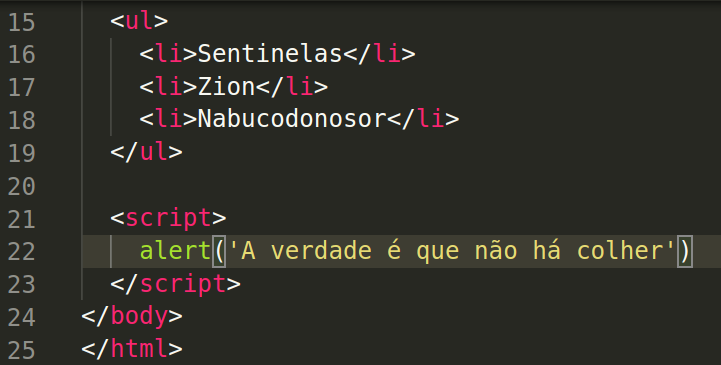
\includegraphics[scale=.5]{imgs/alert-code.png}
    \caption{Código JavaScript dentro do arquivo HTML.}
    \label{fig:alert-code}
\end{figure}



Ou para testar pedacinhos de código, basta digitá-los na aba console do Chrome DevTools.


Ao salvar o arquivo, uma caixa de diálogo deve aparecer no navegador com
a mensagem igual à string presente na chamada da função \texttt{alert}.
Na verdade, o elemento \texttt{script} pode ser posicionado em qualquer
lugar, mas é boa prática colocar no final de \texttt{body} pois o código
JS só é carregado depois que todo o código HTML já foi carregado na
página (na marioria dos casos). Vamos entender isso melhor mais pra frente.


\begin{figure}[h!]
    \centering
    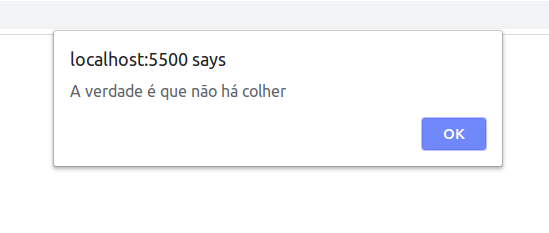
\includegraphics[scale=.5]{imgs/alert-page.png}
    \caption{Resultado do código.}
    \label{fig:alert-page}
\end{figure}


Daqui para frente, sempre deixe o painel do Chrome aberto no console
quando estiver checando seu código JS. É lá que vão aparecer os erros.

\subsection{Tipos de dado}
Temos números inteiros, reais, strings e listas. As lista funcionam de modo semelhante aos vetores em C.

\begin{figure}[h!]
    \centering
    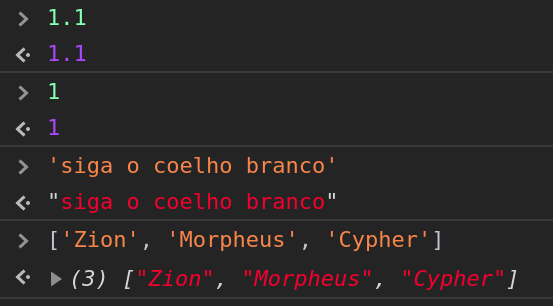
\includegraphics[scale=.5]{imgs/data-types.png}
    \caption{Tipos de dado.}
    \label{fig:data-types}
\end{figure}


\subsubsection{Declaração de variáveis}

Existem três formas de declarar variáveis. De forma muito breve, elas
são:

\texttt{var minhaVariavel = 1}: é a forma menos restrita de se fazer
uma declaração. Assim, \texttt{minhaVariavel} pode mudar de valor e até
ser redeclarada.

\texttt{let segundaVariavel = `uma string'}:
é um pouco mais restrito que \texttt{var}. \texttt{segundaVariavel} não
pode ser redeclarado, mas pode ter seu valor  reatribuído. Além disso,
\texttt{segundaVariavel} só existe até o fim do escopo, ou seja, dentro
do espaço delimitado por \texttt{\{} e \texttt{\}}.

\texttt{const outraVariavel = 0}: é a declaração mais restrita. Não
pode ser redeclarada e nem reatribuída. Assim, \texttt{outraVariavel++}
não funcionaria porque é uma reatribuição de valor. Apesar da palavra
\texttt{const} expressar a ideia de que a variável é constante (no
sentido de que ela não pode mudar de forma alguma), essa ideia está
equivocada. Vamos entender isso um pouco mais pra frente.
\texttt{outraVariavel} também está limitada ao escopo em que foi
declarada.

Se o leitor quiser saber mais sobre o assunto, ele pode ler \href{https://www.alura.com.br/artigos/entenda-diferenca-entre-var-let-e-const-no-javascript}{aqui}.

Nesse tutorial, vamos usar \texttt{const} e \texttt{let}.

Além disso, note que não precisamos especificar a variável do tipo
string, inteiro ou float. Isso acontece porque JS é uma linguagem
fracamente tipada, diferente do C, Java e Python. Quem executa o JS
(no nosso caso,  o próprio navegador) descobre na hora da execução o 
tipo da variável. Assim, não é necessário especificar os tipos dos 
argumentos nas declarações de função.

\begin{quote}
\textbf{Boa prática:} \textit{ser consistente na nomeação de variáveis e funções}
\end{quote}

Por padrão, a convenção usada para nomear variáveis e funções no JS é o
\href{https://en.wikipedia.org/wiki/Camel_case}{camelCase}. De maneira
geral, ela diz que devemos juntar todas a palavras (sem usar
\texttt{\_}) do nome e usar letra maiúscula na primeira letra de cada
palavra.

Deixar de seguir essa convenção não irá causar bugs, mas ainda é
aconselhável utilizar dela para ser mantida a consistência.
\emph{Códigos que são consistentes são mais fáceis de ler, entender e
continuar ou refatorar depois}. É algo que valorizamos no mundo da programação.

Em outras, linguagens como C ou Python, é mais comum o programador
escolher qual convenção usar (camelCase, PascalCase, snake\_case,
kebab-case). O princípio é escolher uma e mantê-la até o final.

\begin{quote}
\textbf{Dica:} \textit{escreva código em inglês e comentários na língua que for
mais confortável}
\end{quote}

Esse é um ponto de muita preferência pessoal. Para este que vos escreve,
escrever código em inglês é mais uma maneira de manter a consistência,
nesse caso com a própria linguagem que é dada para nós em inglês. Se o
leitor ainda optar por usar português, desde que faça assim até o final,
não haverá dificuldades.

\subsubsection{Condicionais e laços de repetição}
São muito semelhantes ao que já usamos em C:

\begin{figure}[h!]
    \centering
    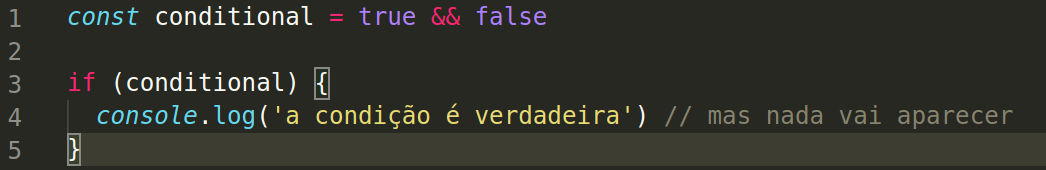
\includegraphics[scale=.4]{imgs/conditional.png}
    \caption{Exemplo de condicional.}
    \label{fig:conditional}
\end{figure}

 \texttt{console.log} é a função que imprime na tela.

\begin{figure}[h!]
    \centering
    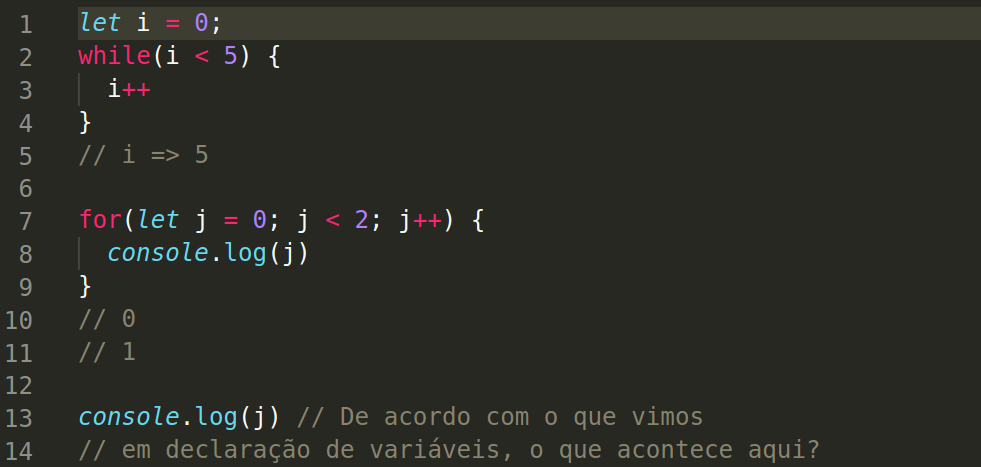
\includegraphics[scale=.4]{imgs/loops.png}
    \caption{Exemplo de laço de repetição com \texttt{while} e \texttt{for}.}
    \label{fig:loops}
\end{figure}


\newpage
\subsubsection{Funções}
Existem 
\href{https://developer.mozilla.org/en-US/docs/Web/JavaScript/Reference/Functions}{várias formas}  
de se declarar uma função. Vamos ver três nesse tutorial.

\begin{figure}[h!]
    \centering
    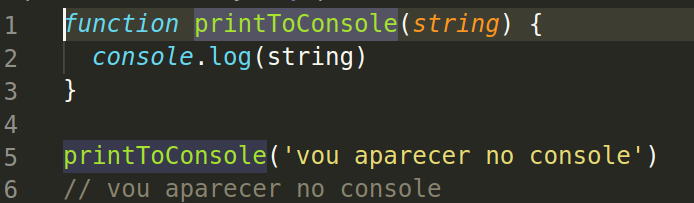
\includegraphics[scale=.4]{imgs/function1.png}
    \caption{ Primeira forma de declarar uma função }
    \label{fig:function1}
\end{figure}

Nesse caso, declaramos uma função com o nome \texttt{printToConsole}.
Quando necessário, perte \texttt{F5} para apagar as variáveis do navegador a cada trecho
exemplo apresentado. Assim, você poderá escrever os código do jeito que
estão nos exemplos (usando \texttt{const}).


\begin{figure}[h!]
    \centering
    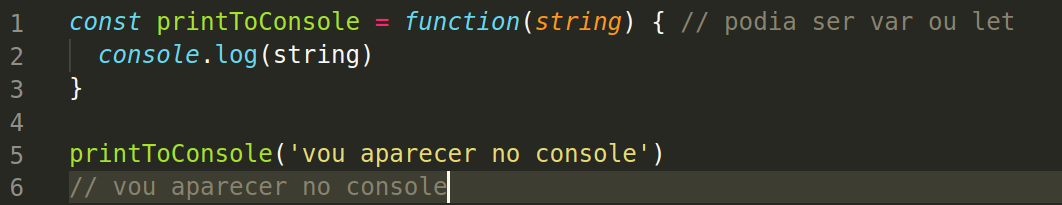
\includegraphics[scale=.4]{imgs/function2.png}
    \caption{ Segunda forma de declarar uma função }
    \label{fig:function2}
\end{figure}

Nesse segundo caso, a atribuímos a referência de uma função anônima à
variável \texttt{printToConsole}. Função anônima porque o que vem depois
de \texttt{=} é uma função por si só, mas \emph{sem nome} e que funciona
também. Entretanto, se não atribuirmos a referência de uma função
anônima a nenhuma variável ou não passarmos ela como argumento de
\emph{outra} função, a função anônima se perde. Vamos voltar nesse
detalhe mais à frente.


\begin{figure}[h!]
    \centering
    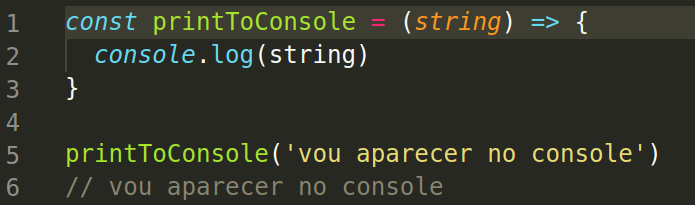
\includegraphics[scale=.4]{imgs/function3.png}
    \caption{ Terceira forma de declarar uma função }
    \label{fig:function3}
\end{figure}

O terceiro caso usa a sintaxe de 
\href{https://www.sitepoint.com/es6-arrow-functions-new-fat-concise-syntax-javascript/}{arrow functions}. 
É uma adição recente no JS e muito utilizada por permitir ao programador escrever menos código em certas situações.

Nesse treinamento vamos nos ater à primeira e à segunda forma.

\newpage
\subsubsection{Objetos}
Tudo no JS é objeto. Até funções são objetos e essa frase vai morrer
aqui. Grosseiramente, podemos comparar objetos do JS aos structs do C.
De maneira ainda mais grosseira, objetos são variáveis que podem possuir
outras variáveis e funções dentro dela. Essas outras variáveis que estão
dentro são chamadas de propriedades. As propriedades e funções acessadas
através do \texttt{.}.

\begin{figure}[h!]
    \centering
    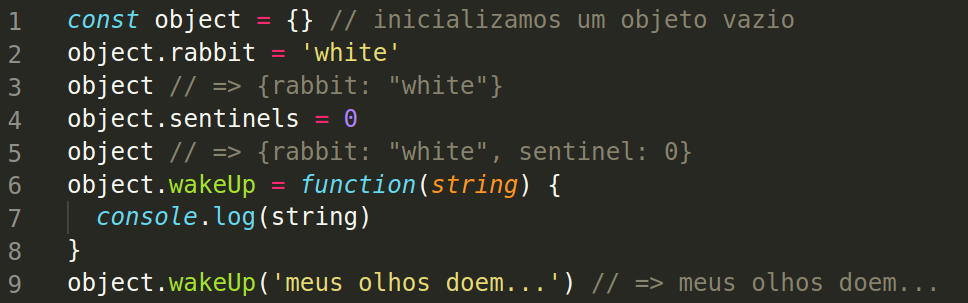
\includegraphics[scale=.4]{imgs/empty-object.png}
    \caption{ Exemplo de construção de um objeto em JS. }
    \label{fig:empty-object}
\end{figure}


\subsubsection{DOM}
Document Object Model. É mais um objeto que é dado para nós quando
utilizamos JS em um navegador. Através dele podemos acessar e modificar
\emph{todos} os elementos HTML que foram carregados na página.
Novamente, DOM é a representação - em forma de objeto - dos elementos
HTML na página. Não vamos muito mais afundo que isso, mas se quiser
saber mais, leia
\href{https://developer.mozilla.org/en-US/docs/Web/API/Document_Object_Model/Introduction}{aqui}.

Assim como no CSS, existe um processo de \textbf{selecionar} e
\textbf{modificar} 
os elementos através de funções (ou métodos) da DOM,
que é dada a nós no objeto global \texttt{document}. Para selecionar um
elemento podemos usar, dentre várias outros, o método
\texttt{querySelector} para selecionar a primeira correspondência. Ainda
utilizando o conteúdo do arquivo \texttt{index.html}: \\

\begin{lstlisting}[language=C++]
document.querySelector(`h1`) // => <h1>Bem vindo ao Deserto Da Realidade</h1>
\end{lstlisting}


\hfill

Nota: vou usar códigos escritos a partir de agora porque tirar screenshots está impraticável :/.

Note que o retorno da função \emph{não} é uma string (confira no console do navegador). É outro objeto
DOM, impresso na tela como representação do primeiro elemento
\texttt{h1} encontrado na página. Podemos guardar a referência para esse
elemento em uma variável. \\


\begin{lstlisting}[language=C++]
const h1 = document.querySelector('h1')
h1 // => <h1>Bem vindo ao Deserto Da Realidade</h1>
\end{lstlisting}

\hfill

Para selecionar um elemento com classe ou uma id, o processo é semelhante ao CSS: \\


\begin{lstlisting}[language=C++]
document.querySelector('.my-class') // para classes
document.querySelector('#my-id') // para id
\end{lstlisting}

\hfill

Uma vez selecionado o(s) elemento(s) de interesse, podemos modificar suas estilizações (regras) através da propriedade \texttt{style}. Dê uma olhada no seu console digitando:\\

\begin{lstlisting}[language=C++]
const h1 = document.querySelector('h1')
h1.style
\end{lstlisting}

\begin{figure}[h!]
    \centering
    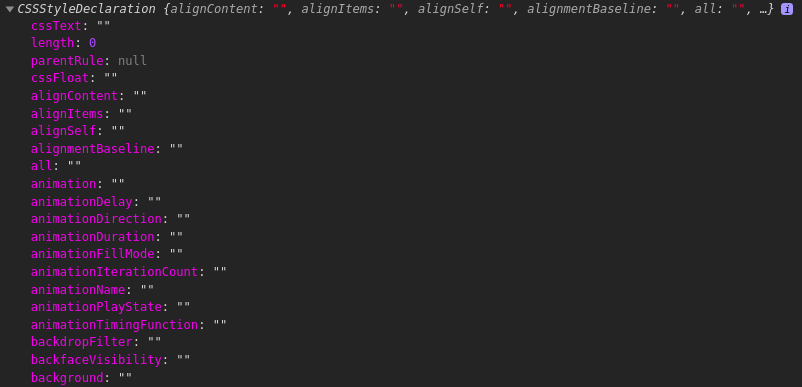
\includegraphics[scale=.5]{imgs/style-prop.png}
    \caption{Imprimindo na tela a propriedade \texttt{style}.}
    \label{fig:style-prop}
\end{figure}


O que você deve ver é algo parecido com o resultado da Firgura \ref{fig:style-prop}. Nessa propriedade estão todas as estilizações configuradas em código JS através da propriedade \texttt{style}, como no próximo exemplo. Leia mais sobre isso \href{https://developer.mozilla.org/en-US/docs/Web/API/ElementCSSInlineStyle/style}{aqui}, na parte ``Getting style information''. Além disso, Note que as propriedades da propridade \texttt{style} são strings.

Para alterar uma estilização (regra) basta atribuir um valor em string:\\


\begin{lstlisting}[language=C++]
h1.style.color = 'red' // depois dessa linha o h1 deve ficar 
                       // vermelho no seu navegador.
\end{lstlisting}

\hfill

O mesmo resultado seria obtido se fosse feito\\

\begin{lstlisting}[language=C++]
h1.style.color = '#ff0000' 
// ou
h1.style.color = 'rgba(255, 0, 0)'
\end{lstlisting}

\hfill


Dessa forma todas as regras que escrevemos em um arquivo CSS também podem ser aplicadas em JS.

Podemos mudar seu conteúdo também:\\

\begin{lstlisting}[language=C++]
h1.innerText = 'He is beginning to believe'
\end{lstlisting}
\hfill

O elemento h1 no seu navegador deve ter o seu conteúdo diferente agora.

\newpage
\subsubsection{ \texttt{createElement} }
Podemos também criar qualquer elemento HTML através do JavaScript: \\

\begin{lstlisting}[language=C++]
const h1 = document.createElement('h1')
h1.innerText = 'Follow th white rabbit'
h1 // => <h1>Follow th white rabbit</h1>
\end{lstlisting}
\hfill

Na linha 1 criamos um elemento DOM que é um h1 e atribuímos sua referência à variável \texttt{h1}
. Em seguida colocamos um texto no conteúdo de \texttt{h1} e depois o elemento é impresso no console.

Naturalmente, nada acontece na página porque nós apenas criamos um elemento, mas não ele não foi colocado em lugar algum. Para inserir um elemento no código HTML precisamos especificar um ponto de entrada, que é geralmente outro elemento da DOM. Vamos inserir o \texttt{h1} no elemento body do código HTML usando o método \texttt{append}.\\

\begin{lstlisting}[language=C++]
const body = document.querySelector('body')

body.append(h1) // h1 que foi criado anteriormente

\end{lstlisting}
\hfill

O leitor deve notar que outro título foi adicionado ao \textit{final} da página, o mesmo título criado com \texttt{createElement('h1')}.


\subsubsection{\texttt{setInterval} }
Se quisermos que algum trecho de código seja executado com  certa frequência, podemos usar a função \texttt{setInterval}. Essa função recebe pelo dois argumentos: o primeiro deve ser a referência pra uma função que será executada periodicamente e o segundo é o tempo em milissegundos. \\

\begin{lstlisting}[language=C++]
function printWakeUp() {
    console.log('wake up')
}

setInterval(printWakeUp, 1000)
\end{lstlisting}
\hfill


\begin{figure}[h!]
    \centering
    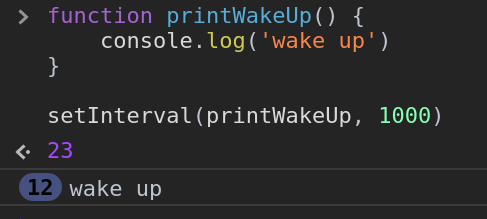
\includegraphics[scale=.5]{imgs/setInterval-wakeUp.png}
    \caption{ Resultado da função. }
    \label{fig:setInterval-wakeUp}
\end{figure}

Pode obter o mesmo resultando fazendo o seguinte:

\begin{figure}[h!]
    \centering
    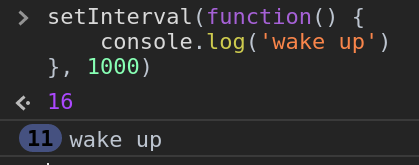
\includegraphics[scale=.5]{imgs/setInterval-anon-function.png}
    \caption{ Resultado da função. }
    \label{fig:setInterval-anon-function}
\end{figure}

Nesse caso, estamos usando uma função anônima. Como a referência para a função a ser executada periodicamente só é usada para a função \texttt{setInterval}, ela não precisa de um nome.

Com isso podemos, por exemplo, aumentar periodicamente o tamanho da fonte de um elemento  \\

\begin{lstlisting}[language=C++]
const h1 = document.querySelector('h1')
h1.style.fontSize = '10px'

function incrementSize() {
    h1.style.fontSize = parseInt(h1.style.fontSize) + 1 + 'px'
}

setInterval(incrementSize, 1000)
\end{lstlisting}
\hfill

Estamos conhecendo \texttt{parseInt} agora. O que ela faz é retornar o primeiro inteiro encontrado em uma string. 

Você pode achar estranho também o que está acontecendo na linha 5. Estamos somando dois inteiros e concatenando com uma string. Bem, isso é permitido no JS. O resultado disso é convertido pra string automaticamente.




\subsubsection{Desafio}
Fica aí um desafio: faça o título da página mudar pra uma cor aleatória a cada meio segundo.

Lembre-se que o Google é seu amigo. Pesquise como gerar números aleatórios em JavaScript.